\chapter{Future Work}

The question as per \cite{Turian2022HEAR:Representations} or \cite{Li2023MERT:Training} remains if such general-purpose audio representation can mimic human hearing. That is a "thorn in our side" that we will pursue.

transforms
stems
different takes
k-fold cross validation
hyper-params: kernel size 0.005 times the sample rate
larger representation layer
Loss function margin. A margin of 0.2 can be a starting point, but it might not be the best value for every task. It's recommended to experiment with different values and choose the one that provides the best performance on your validation set.

Utilize the dB-scale Mel-spectrum magnitude of audio as input data; it is a popular choice for input representation in music-related tasks when applying CNNs, as has been demonstrated in various studies \cite{Kim2020OneStrategies}. While raw audio is the most meaningful audio representation, it's been reported that dB-scale Mel-spectrum frequency-domain summarization, grounded in psycho-acoustics, is computationally efficient and challenging to replicate solely through data-driven methods \cite{Kim2020OneStrategies}; therefore, a trade-off that looks worthy of being explored.

Visual and listening evaluation: 2D or 3D latent space visualization as per \ref{fig:manifold}. Arranging the embedding space in a visual display to evaluate the clustering of this sophisticated musical content to see to what extent they consider sonic attributes. 

\begin{figure}[ht]
    \centering
    \scalebox{1.2}{

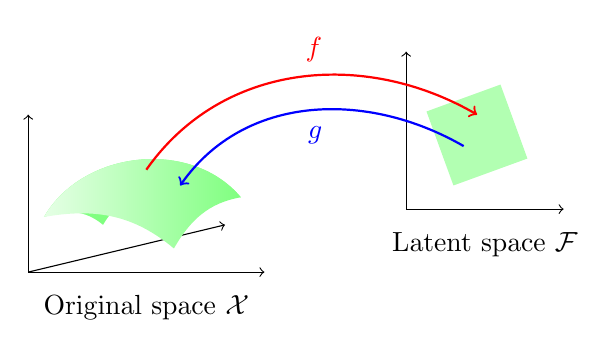
\begin{tikzpicture}
\centering
\draw[->] (0, 0) -- ++(0, 2);
\draw[->] (0, 0) -- ++(2.5, 0.6);
\draw[->] (0, 0) -- ++(3, 0) node[midway, below, yshift=-0.5em]
    {Original space ${\cal X}$};

\draw[fill=green!50, draw=none, shift={(0.2, 0.7)},scale=0.5]
  (0, 0) to[out=20, in=140] (1.5, -0.2) to [out=60, in=160]
  (5, 0.5) to[out=130, in=60]
  cycle;

\shade[thin, left color=green!10, right color=green!50, draw=none,
  shift={(0.2, 0.7)},scale=0.5]
  (0, 0) to[out=10, in=140] (3.3, -0.8) to [out=60, in=190] (5, 0.5)
    to[out=130, in=60] cycle;

  \draw[->] (4.8, 0.8) -- ++(0, 2);
  \draw[->] (4.8, 0.8) -- ++(2, 0) node[midway, below, yshift=-0.5em]
      {Latent space ${\cal F}$};

  \draw[thin, fill=green!30, draw=none, shift={(5.4, 1.1)}, rotate=20]
    (0, 0) -- (1, 0) -- (1, 1) -- (0, 1) -- cycle;

  \draw[thick,->,red]
    (1.5, 1.3) to [out=55, in=150] node[midway, above, xshift=6pt, yshift=2pt]
    {$f$} (5.7, 2);

  \draw[thick,->,blue] (1.5, 1.3) ++(4.03, 0.3) to [out=150, in=55]
    node[midway, below, xshift=2pt, yshift=-2pt] {$g$} ++(-3.6, -0.5);

\end{tikzpicture}}
    
    \caption[Dimensionality reduction and latent space representation \cite{tikz}.]{\small{Dimensionality reduction and latent space representation: Mapping between the original high-dimensional space ${\cal X}$ and the lower-dimensional latent space ${\cal F}$ using functions $f$ and $g$.}}
    \label{fig:manifold}
\end{figure}


\newpage